%TCIDATA{LaTeXparent=0,0,cap_RevisaoBibliografica.tex}

\section{Simulação Numérica de Reservatórios}

A simulação numérica de um reservatório é, segundo Peaceman, é o processo de inferência do comportamento do reservatório real dada a performance obtida de um modelo do mesmo, matemático ou físico (em escala laboratorial). Um modelo matemático de reservatório pode ser enxergado como um conjunto de equações diferenciais parciais, juntamente com as condições de contorno adequadas, que podem ser utilizadas para descrever satisfatoriamente os processos físicos importantes que ocorrem no sistema real.

Os processos que ocorrem em um reservatório são basicamente transporte de fluidos e transferência de massa; até três fases imiscíveis (óleo, gás e água) fluem simultaneamente, enquanto que o transporte de massa se dá entre as fases (notadamente entre o óleo e o gás). A gravidade, a capilaridade e as forças viscosas são também importantes no processo de vazão dos fluidos \cite{simres}.

Segundo Rosa, a primeira etapa de uma simulação numérica é formular o problema físico a ser representado matematicamente; em seguida são feitas suposições e simplificações compatíveis com o grau de sofisticação esperado do modelo, levando-se à formulação das equações matemáticas que descrevem o problema desejado, considerando-se as hipóteses adotadas. O passo seguinte é a resolução das equações e análise da solução obtida; posteriormente, a validade do simulador é verificada através da calibração com uma solução existente --- por exemplo, comparam-se os resultados obtidos do simulador numérico com soluções analíticas, resultados reais ou com resultados obtidos de modelos físicos de laboratório (dados experimentais). Caso o simulador seja considerado válido, o mesmo estará pronto para ser utilizado na simulação do fenômeno desejado; caso contrário, volta-se para um novo ciclo em que são revistas as hipóteses adotadas ou até a conceituação do modelo físico \cite[p. 520]{engres}. A Figura \ref{fig:rev_simuesq} esquematiza um desenvolvimento básico de um simulador numérico qualquer, enquanto que a Figura \ref{fig:rev_simuex} mostra uma comparação de resultados entre diferentes simuladores existentes, exemplificando o uso da calibração com soluções já obtidas para se validar um simulador de reservatório. 

\begin{figure}[!ht]
\centering
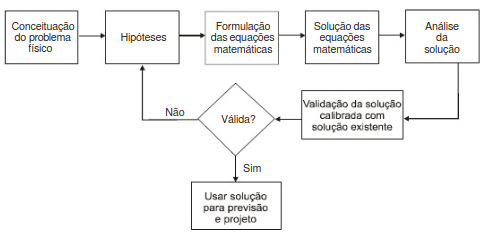
\includegraphics[width=.75\textwidth]{figs/revisao/revisao_simuesq.png}
\caption{Esquema básico de desenvolvimento de um simulador numérico de reservatório \cite[p. 519]{engres}.}\label{fig:rev_simuesq}
\end{figure}

\begin{figure}[!ht]
\centering
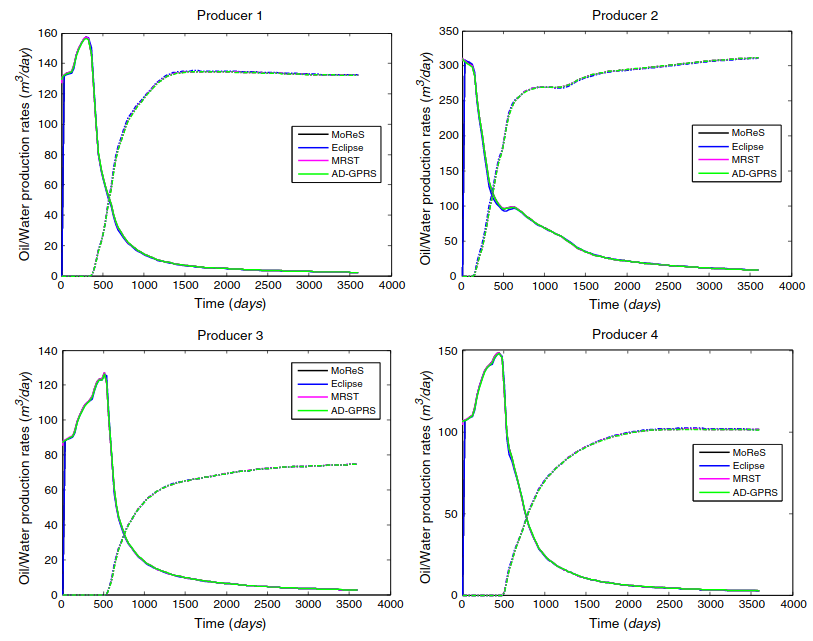
\includegraphics[width=.75\textwidth]{figs/revisao/revisao_simuex.png}
\caption{Exemplo de comparação de dados entre simuladores de vazão de água e de óleo de um modelo \cite{eggM}.}\label{fig:rev_simuex}
\end{figure}

\subsection{Leis Físicas Consideradas}

No caso de um simulador de reservatórios, as seguintes leis físicas básicas normalmente são consideradas, dependendo do tipo de simulador\footnote{Ver \cite[p. 520]{engres}}:

\begin{itemize}
\item Lei da conservação de massa;
\item Lei da conservação de energia;
\item Lei da conservação de \textit{``momentum''} (Segunda Lei de Newton):
\begin{equation}
\sum F = \frac{\partial M}{\partial t},
\end{equation}
onde $F$ representa uma força e $M = mv$ o \textit{``momentum''}, com $m$ sendo a massa e $v$ a velocidade.
\end{itemize}

Além das leis básicas da física, faz-se necessário o uso de várias leis, dependendo do simulador, que governam o comportamento dos fluidos envolvidos e a propriedade do reservatório estudado, apresentadas nas subseções a seguir\footnote{Os teoremas apresentados se encontram em \cite[pp. 520-522]{engres}}. Combinado-se as equações correspondentes às leis básicas, obtém-se uma equação diferencial parcial que rege o comportamento das variáveis dependentes em função das variáveis independentes e dos parâmetros do sistema. Como normalmente a equação obtida é não-linear, ela é, consequentemente, é resolvida por métodos númericos; daí a nomenclatura \textit{simulação numérica de reservatórios}.

\subsubsection{Fenômenos de Transporte}

\begin{theorem}[Lei de Darcy]
Na Lei de Darcy, ou lei do fluxo ``laminar'' ou Darcyano, a velocidade do fluxo viscoso de um fluido em meio poroso é dada por
\begin{equation}
	v_s = -\frac{k_s}{\mu} \frac{\partial\Phi}{\partial s},
\end{equation}
onde $k$ é a permeabilidade efetiva do meio ao fluido considerado, $\mu$ é a viscosidade do fluido, $\Phi$ é o potencial de fluxo e $s$ é a trajetória de fluxo.
\end{theorem}

\begin{theorem}[Lei de Forchheimer]
Também conhecida como lei do fluxo ``turbulento'' ou não-Darcyano, é utilizada para fluxos turbulentos, notadamente de gás; o gradiente de pressão é dado por
\begin{equation}
	-\frac{dp}{ds} = \frac{\mu}{k_s}v_s - \beta\rho v_s^2,
\end{equation}
onde $\rho$ é a massa específica do fluido e $\beta$ é o coeficiente de resistência inercial ou de fluxo não-Darcyano. 
\end{theorem}

\begin{theorem}[Lei de Fourier]
Durante um fenômeno de transporte de calor por condução, o fluxo de calor é dado por
\begin{equation}
	q_s = -k'\frac{\partial T}{\partial s},
\end{equation}
em que $k'$ é a condutividade térmica do meio e $T$ é a temperatura.
\end{theorem}

\begin{theorem}[Convecção]
O fluxo de calor no caso de tranporte por convecção é dado por
\begin{equation}
	q_s = c_p v_s (T - T_0),
\end{equation}
onde $c_p$ é a capacidade calorífica do fluido à pressão constante, $v$ a velocidade do fluido e $T_0$ uma temperatura de referência.
\end{theorem}

\subsubsection{Equações de Estado}
As principais equações de estado envolvidas na simulação do comportamento de um reservatório de petróleo são as que lidam com fluidos (líquidos ou gasosos) e rochas porosas. No caso de fluidos líquidos, tem-se a seguinte definição:

\begin{definition}
A compressibilidade isotérmica de um fluido é dada por
\begin{equation}
	c = -\frac{1}{V}\frac{\partial V}{\partial p} = \frac{1}{\rho}\frac{\partial \rho}{\partial p},
\end{equation}
em que $V$ é o volume, $p$ é a pressão e $\rho$ é a massa específica do fluido. Há algumas relações especiais para situações particulares:
\begin{itemize}
\item Líquidos de compressibilidade constante: $\rho = \rho_0 e^{c(p-p_0)}$.
\item Líquidos de compressibilidade constante e pequena: $\rho = \rho_0 \left[1+c\left(p-p_0\right)\right]$.
\end{itemize}
\end{definition}

Quando se trata de estudar o estado de um gás, se aplica a lei dos gases:
\begin{equation}\label{eq:gaslaw}
	\rho = \frac{pM}{ZRT}.
\end{equation}

A Equação \eqref{eq:gaslaw} pode ser aplicada tanto no caso de um gás real quanto de um gaś ideal; nela, $\rho$ é a massa específica do gás, $p$ é a pressão, $M$ é a massa molecular, $R$ é a constante universal dos gases, $T$ é a temperatura e $Z$ é o fator de compressibilidade do gás; no caso de um gás ideal, tem-se $Z = 1$.

Por fim, para se representar o comportamento da rocha, utiliza-se a equação da chamada compressibilidade efetiva:
\begin{equation}
	c_f = \frac{1}{\phi} \frac{\partial\phi}{\partial p},
\end{equation}
onde $c_f$ é a compressibilidade efetiva efetiva da formação e $\phi$, sua porosidade.

Além das leis até aqui citadas, cabe ressaltar que outras podem ser utilizadas em caso de simulações de fenômenos específicos, como injeção de vapor, injeção de polímeros, além de outros métodos empregados na produção de petróleo.

\subsection{Tipos de Simuladores}
Segundo Rosa, os simuladores de reservatórios podem ser classificados em função de três critérios básicos: o tratamento matemático utilizado, o número de dimensões consideradas e o número de fases admitidas. Em relação à matemática do simulador, os simuladores podem ser classificados em: 

\begin{itemize}
	\item \textbf{Modelo Beta ou volumétrico:} É também conhecido como \textit{black oil}; nesse modelo, são consideradas as funções de pressão e da temperatura do reservatório. Além disso, cada fase presente no reservatório (água, óleo e/ou gás) é admitida como constituída por apenas um componente, mesmo que, na prática, o óleo seja composto por vários hidrocarbonetos, além de impurezas.
	\item \textbf{Modelo composicional:} Além de considerar a pressão e a temperatura do reservatório, também se admite as composições das diversas fases que estejam presentes no meio poroso. Ao contrário do \textit{black oil}, por exemplo, o óleo passa a ser tratado pelos seus vários hidrocarbonetos de que é composto, tais como $C_1$, $C_2$, $C_3$, etc. Porém, como o número de componentes no óleo é grande, alguns hidrocarbonetos são agrupados nos chamados \textit{pseudocomponentes}; a utilização dessa abordagem reduz o tempo computacional necessário ao modelo, uma vez que um tratamento mais rigoroso poderia tornar impraticável a simulação composicional.
	\item \textbf{Modelo térmico:} É utilizado quando é necessário considerar os efeitos de variações térmica no interior do reservatório --- por exemplo, quando se estuda a aplicação de métodos térmicos de recuperação secundária, como injeção de vapor, injeção de água quente ou combustão \textit{in situ}. Como os modelos térmicos tratam situações complexas, eles são necessariamente composicionais.
\end{itemize}

Quanto ao número de dimensões, os simuladores são classificados de acordo com o número de dimensões nas quais se admite fluxo. Neste sentido, eles podem ser classificados em \textit{unidimensionais} (Figura ...), \textit{bidimensionais} (Figura ...) e \textit{tridimensionais} (Figura ...). Por fim, os simuladores numéricos podem ser classificados de acordo com o número de fases: \textit{monofásicos}, caso haja apenas uma fase (no caso de água, se trata de um aquífero); \textit{bifásicos}, quando há duas fases presentes (água e óleo, no caso de reservatórios de óleo, ou água e gás, nos reservatórios de gás); e \textit{trifásicos}, no caso da existência de três fases (água, óleo e gas)\footnote{A classificação dos modelos de simulação podem ser encontradas em \cite[pp. 517--519]{engres}}.

%TODO : Insira as figuras AQUI!

É importante que, ao se escolher um simulador numérico para se resolver problemas de engenharia de reservatório, se considere vários fatores, a saber: o tipo de estudo a ser feito, tipo e características do reservatório e dos fluidos presentes, quantidade e qualidade dos dados, o detalhamento necessário do estudo e os recursos computacionais disponíveis \cite[p. 519]{engres}. Por exemplo, é impraticável o uso de modelos composicionais em computadores cuja capacidade seja comparável a um computador pessoal de alto desempenho, devido à complexidade dos cálculos envolvidos. Por outro lado, por sua simplicidade, um modelo \textit{black oil} poderia ser considerado, respeitando-se ao máximo as características do reservatório estudado.

\subsection{Uso de Simuladores Numéricos para Estudos de Reservatórios}

O uso de simuladores numéricos torna possível analisar o comportamento de um reservatório ao longo do tempo, dado um esquema de produção. Dessa forma, pode-se obter, por exemplo, as condições ótimas de produção, além de se determinar como a injeção de diferentes tipos de fluidos ou outros métodos de EOR afetam o sistema simulado, determinar o efeito da localização dos poços na recuperação de óleo e/ou gás e analisar a influência de diferentes vazões de produção e/ou injeção. O simulador obtém seus resultados de informações de natureza geológica, propriedades da rocha e dos fluidos presentes no meio poroso, históricos de produção (vazões e/ou produções acumuladas de óleo e água) e de pressão, e outras informações a respeito dos poços de petróleo, assim como as características de completação \cite[pp. 522--523]{engres}. A Figura \ref{fig:revisao_simsec1} ilustra a aplicação de simuladores numéricos para engenharia de reservatórios.

\begin{figure}[!ht]
	\centering
	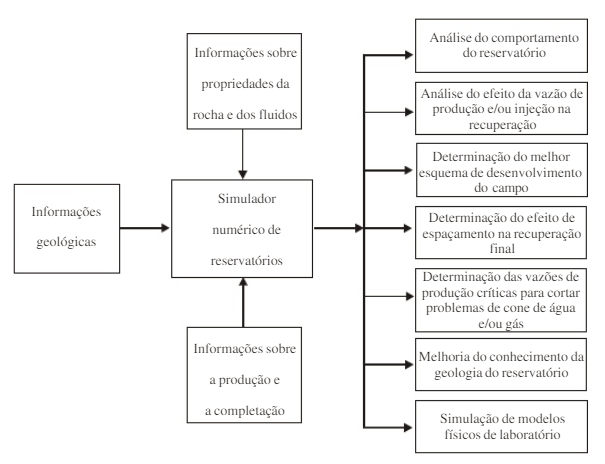
\includegraphics[width=.6\textwidth]{figs/revisao/revisao_simsec1}
	\caption{Aplicação de simuladores numéricos em reservatórios \cite[p. 522]{engres}}
	\label{fig:revisao_simsec1}
\end{figure}  

